\documentclass[a4paper]{article}

%% Language and font encodings
\usepackage[utf8]{inputenc}
\usepackage[ngerman]{babel}
\usepackage[T1]{fontenc}
\usepackage{caption}

%% Sets page size and margins
\usepackage[a4paper,top=3cm,bottom=2cm,left=3cm,right=3cm,marginparwidth=1.75cm]{geometry}

%% Useful packages
\usepackage{amsmath}
\usepackage{graphicx}
\usepackage{subfig}
\usepackage{tabularx}
\usepackage[style=nature]{biblatex}
\usepackage[colorinlistoftodos]{todonotes}
\usepackage[colorlinks=true, allcolors=blue]{hyperref}
\usepackage{float}
\usepackage{textcomp}



\addbibresource{references.bib}

\title{Praktikum Neurobiologie - Protokoll 3}

\author{Cedric Laier, Tilman Mehl}


\begin{document}
%Titelpage Modell: https://www.latextemplates.com/template/formal-book-title-page
\begin{titlepage} % Suppresses headers and footers on the title page

	\centering % Centre everything on the title page
	
	\scshape % Use small caps for all text on the title page
	
	\vspace*{\baselineskip} % White space at the top of the page
	
	%------------------------------------------------
	%	Title
	%------------------------------------------------
	
	\rule{\textwidth}{1.6pt}\vspace*{-\baselineskip}\vspace*{2pt} % Thick horizontal rule
	\rule{\textwidth}{0.4pt} % Thin horizontal rule
%	{\LARGE THE BIG BOOK\\ OF\\ \LaTeX ~TEMPLATES\\} % Title
	\vspace{0.75\baselineskip} % Whitespace above the title
	{\LARGE Neurosim - Computersimulation von Nervensignalen} {\\Protokoll zum Praktikum Neurobiologie für Bioinformatiker\\ am 21.01.2019} % Title

	
	\vspace{0.75\baselineskip} % Whitespace below the title
	
	\rule{\textwidth}{0.4pt}\vspace*{-\baselineskip}\vspace{3.2pt} % Thin horizontal rule
	\rule{\textwidth}{1.6pt} % Thick horizontal rule
	
	\vspace{2\baselineskip} % Whitespace after the title block
	
	\vspace{2.0\baselineskip} % Whitespace before the editors

{\LARGE Gruppe 2}
\vspace{2.5\baselineskip} \\
	
{\LARGE Autoren:}
\begin{itemize}
\item Cedric Laier - \textit{cedric.laier@fu-berlin.de}
\item Tilman Mehl - \textit{tilmanmehl@zedat.fu-berlin.de}
\end{itemize}
\vspace{2.5\baselineskip}

{\LARGE Lehrveranstalter:}
\begin{itemize}
\item  Peter Robin Hiesinger
\item Matthias Wernet
\end{itemize}
\vspace{2.5\baselineskip}

{\LARGE Tutoren:}
\begin{itemize}
\item Lisa
\item Johannes
\item Claudia
\end{itemize}
	
\end{titlepage}
\section{Einleitung}
Inhalt des Praktikumstages war die Simulation von grundlegenden elektrophysiologischen Experimenten mit Neurosim\cite{Neurosim}. Konkret wurde betrachtet: \vspace{1.0\baselineskip}
\begin{itemize}
    \item Auswirkung sich ändernder Ionenkonzentration auf das Ruhemembranpotential
    \item Zusammenhang zwischen Reizstärke und Frequenz von Aktionspotentialen
    \item Aktivierung von spannungsabhängigen K\textsuperscript{+} und Na\textsuperscript{+}-Kanälen
    \item Modellierung neuronaler Netze zur Bewegungswahrnehmung
\end{itemize}
\vspace{1.0\baselineskip}
\subsection{Membran und Potentiale}
Zentrales Betrachtungsobjekt unseres Praktikums ist das Neuron, bzw. deren Membran. Die Zellmembran ist aus einer Doppellipidschicht und Membranproteinen aufgebaut.\\
Die unterschiedliche Verteilung von fünf Arten von Ionen auf den beiden Seiten der Membran beeinflusst das Membranpotenzial, also die elektrische Spannung zwischen Extrazellulär- und Intrazellulärraum. Für jedes Ion lässt sich mittels der Nernst-Gleichung ein Gleichgewichtspotenzial berechnen, d.h. eine Spannung die an der Membran anliegen müsste, so dass Ein- und Ausstrom des Ions im Gleichgewicht sind. Bei einer Temperatur von 20\textdegree{}C gilt: \\ \\
\[E_{ion} = 58mV \cdot log\left(\frac{c_o}{c_i}\right)\] \\ \\
Um das gesamte Membranpotential zu ermitteln, müssen alle beteiligten Ionen betrachtet werden. Dies ist mit der Goldmann-Gleichung möglich, bei der alle Ionenkonzentration und -permeabilitäten einbezogen werden. \\ \\
\[V_m = \frac{RT}{F}ln\left(\frac{p_K[K^+]_o + p_{Na}[Na^+]_o + p_{Cl}[Cl^-]_i}{p_K[K^+]_i + p_{Na}[Na^+]_i + p_{Cl}[Cl^-]_o}\right)\] \\ \\
Das Ruhemembranpotenzial ist das Membranpotenzial, wenn keine Erregung vorliegt. Es liegt in der Regel zwischen -90 und -40 mV. Wie an der Goldmann-Gleichung zu erkennen, ist das Ion mit der größten relativen Permeabilität (Kalium) maßgeblich am Ruhemembranpotential beteiligt.\\ \\
Von besonderer Bedeutung für die Funktion der Neuronenmembran ist die Natrium-Kalium-Pumpe und die spannungsabhängigen Natrium- und Kaliumkanäle. Die Natrium-Kalium-Pumpe ist ein aktiver Transporter, der unter ATP Verbrauch 3 Na\textsubscript{+}-Ionen aus der Zelle hinaus, und 2 K\textsuperscript{+}-Ionen in die Zelle hinein befördert. Dadurch wird ständig ein Konzentrationsgradient, sowie ein Spannungsgradient zwischen Intra- und Extrazelluär erhalten. Die spannungsabhängigen Ionenkanäle spielen bei der Erregungsweiterleitung eine wichtige Rolle. Natriumkanäle öffnen sich bei positiver Spannung. Dadurch strömt mehr (positiv geladenes) Natrium in die Zelle ein und löst somit eine Kaskade von sich öffnenden Natriumkanälen aus. Dies führt zu einer raschen Depolarisation der Membran. Zeitgesteuert schließen Natriumkanäle und können in der absoluten Refraktärzeit nicht geöffnet werden. In der darauffolgenden relativen Refraktärzeit liegt der Schwellwert für die Öffnung der Kanäle höher.\cite{CatterallWilliamA2000FICt} Kaliumkanäle öffnen sich ebenfalls abhängig von positiver Spannung, bleiben aber zeitunabhängig so lange geöffnet, bis das Ruhemembranpotential wiederhergestellt ist. In der Zeit bis zum Schließen aller Kaliumkanäle kann das Membranpotential unter das Ruhemembranpotential sinken (Hyperpolarisation).\cite{FaberESLouise2003CPCM} 

\newpage
\noindent Hodgkin und Huxley veröffentlichten 1952 eine Reihe von Artikeln, die ihre Beobachtungen eines Voltage-Clamp Experiments am Riesenaxon eines Tintenfisches beschreiben. Unter anderem wurden darin die an Membranpotential und Erregung maßgeblich beteiligten Ionen ermittelt.\cite{HodgkinHuxley2} \cite{HodgkinHuxleySummary}\\


\subsection{Voltage Clamp}
\noindent Bei dem Voltage-Clamp Experiment handelt es sich um eine Methode um die 
Ionenströme durch die Membran erregbarer Zellen, wie z.B. Neuronen, zu messen
während die Membranspannung auf einem gewissen Level konstant gehalten wird.
Eine Spannungsklemme misst iterativ das Membranpotenzial und ändert dann Membranpotential (Spannung) durch das Hinzufügen des erforderlichen Stroms auf einen gewünschten Wert. 
Dadurch wird die Zellmembran mit einer gewünschten konstanten Spannung "geklemmt", so dass die Spannungsklemme erfassen kann, welche Ströme geliefert werden. Da die an die Zelle angelegten Ströme gleich sein müssen, zeigen die aufgezeichneten Ströme an, wie die Zelle auf Veränderungen des Membranpotentials reagiert. Zellmembranen erregbarer Zellen enthalten viele verschiedene Arten von Ionenkanälen, von denen einige spannungsgesteuert sind. Die Spannungsklemme ermöglicht es, die Membranspannung unabhängig von den Ionenströmen zu manipulieren, so dass die Strom-Spannungs-Verhältnisse von Membrankanälen untersucht werden können. In Abbildung \ref{fig:VersuchsaufbauHH} ist der Versuchsaufbau zu sehen. \\

\begin{figure}[H]
    \centering
    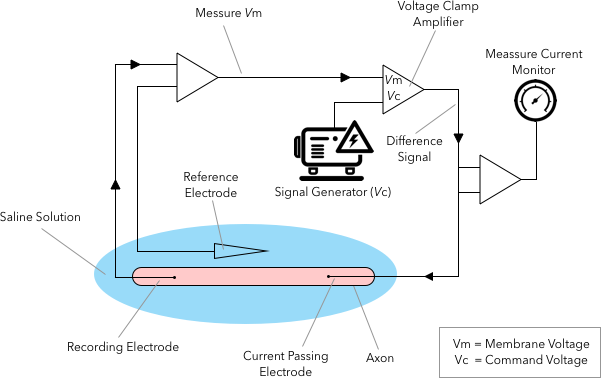
\includegraphics[scale=0.6]{images/Versuchsaufbau_VoltageClamp.png}
    \caption{Versuchsaufbau nach Hodkin - Huxley}
    \label{fig:VersuchsaufbauHH}
\end{figure}
\vspace{2.0\baselineskip}
\subsection{Neuronale Netze und Bewegungswahrnehmung}
Bewegung an sich könnte zwar von einem einzelnen Neuron wahrgenommen werden, allerdings könnte keine Information zur Bewegungsrichtung kodiert werden. Dazu müssen Neuronen zu einem Netz verschaltet werden. Für Bewegungswahrnehmung in eine Richtung ist uns das Barlow-Levick Modell\cite{BarlowLevick} bekannt, für Bewegungswahrnehmung in zwei Richtungen das Reichard-Hassenstein Modell\cite{Reichardt1987}. Beide Modelle basieren auf der Erkenntnis, dass zwei räumlich versetzte Neurone durch die Bewegung zu unterschiedlichen Zeitpunkten erregt werden. Treffen beide Erregungen zeitgleich bei einem dritten Neuron ein, summieren sich die Aktionspotentiale und erregen das dritten Neuron, was als Bewegung wahrgenommen wird.
\newpage
\section{Material und Methoden}
\subsection{Modul Goldmann}
Im ersten Teil des Praktikumstags wurde gemessen, wie eine sich ändernde Kaliumkonzentration auf auf das Membranpotential auswirkt. In Neurosim wurde das Modul Goldmann gestartet. Die Temperatur lag bei 20\textdegree{}C, die Ionenkonzentrationen und Permeabilitäten sind in Tabelle \ref{tab:A1_1} dargestellt.\\
\begin{table}[H]
    \centering
    \caption{Ionenkonzentrationen und Permeabilität}
    \begin{tabular}{|c|c|c|c|}
        \hline
        \textbf{Ion} & \textbf{Relative Permeabilität} & \textbf{Extrazelluläre Konzentration} & \textbf{Intrazelluläre Konzentration}\\
        \hline
        K\textsuperscript{+} & 1.0 & 20 & 400\\
        \hline
        Na\textsuperscript{+} & 0.04 & 440 & 50\\
        \hline
        Cl\textsuperscript{-} & 0.45 & 560 & 75\\
        \hline
    \end{tabular}
    \label{tab:A1_1}
\end{table}

\vspace{1.0\baselineskip}
\noindent Für den Versuch wurde die extrazelluläre K\textsuperscript{+}-Konzentration schrittweise (50mM je Schritt) von 10mM auf 810mM erhöht, und Gleichgewichtspotential für Kalium sowie das Membranpotential gemessen. \vspace{1.0\baselineskip}
\begin{figure}[H]
    \centering
    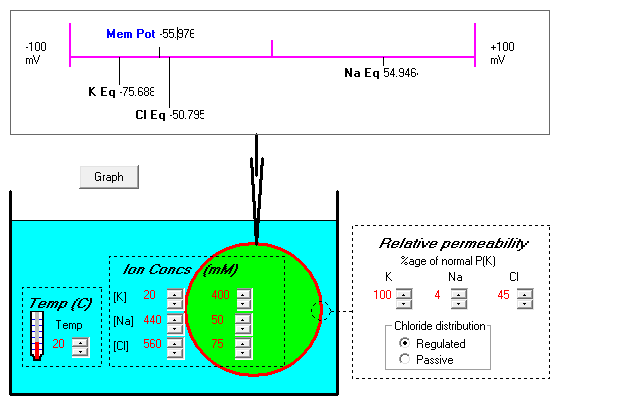
\includegraphics[scale=0.8]{images/Aufgabe1_1_Aufbau.png}
    \caption{Startparameter für Modul Goldmann}
    \label{fig:my_label}
\end{figure}
\noindent Anschließend wurden für einige Beispielwerte von Ionenkonzentrationen und -permeabilitäten mit Hilfe der Nernst'schen Gleichung die jeweiligen Gleichgewichtspotentiale bestimmt. Mit Hilfe der Goldmann Gleichung wurde für die Werte das Membranpotential berechnet.

\subsection{Modul Hodgkin - Huxley (Current Clamp)}
Im Current Clamp Experiment wurde der Zusammenhang zwischen Reizströmen und Frequenz von Aktionspotentialen beobachtet.\\
%2.1 fehlt noch
\\
Für die ersten beiden Experimente wurde die Datei Param2.nrs in Neurosim geladen.\\
Die Temperatur wurde auf 20\textdegree{}C gesetzt. Die Stromamplitude des Stimulus wurde, ausgehend von 50\(\mu\)A, so lange verringert, bis die Schwelle gefunden wurde, bei der zum ersten Mal ein Aktionspotential auftritt. Anschließend wurde der Stimulus schrittweise um 10\(\mu\)A erhöht und die auftretende Maximalspannung sowie die Zeit bis zum auftreten der Maximalspannung notiert.\\
\\
Für das dritte Experiment wurde die Datei IFCURVE.nrs in Neurosim geladen.\\
Die Stromstärke wurde schrittweise von 1\(\mu\)A auf 130\(\mu\)A erhöht. Beobachtet wurden Frequenz und Amplituden der Aktionspotentiale. Die Ionenkonzentrationen lagen innen/außen für Kalium bei 390/10mM und für Natrium bei 70/418mM. Der Stimulus hatte eine Dauer von 90ms und eine Verzögerung von 0,5ms.
\begin{figure}[H]
    \centering
    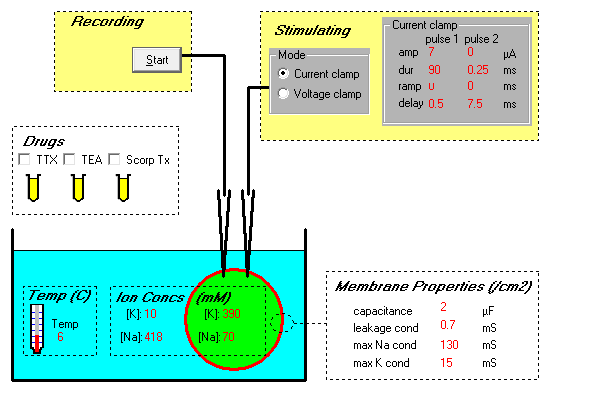
\includegraphics{images/Aufgabe2_4_Setup.png}
    \caption{Ausgangseinstellungen für Frequenz- und Amplitudenmessung bei steigender Stromstärke}
    \label{fig:A2_4_Setup}
\end{figure}
\subsection{Modul Hodgkin - Huxley (Voltage Clamp)}
Im Voltage Clamp Experiment wurde die Aktivierung von spannungsabhängigen Na\textsuperscript{+} und K\textsuperscript{+}-Kanälen beobachtet.\\
\\
In Neurosim wurde die Datei PARAM4.nrs geladen.\\
Das Haltepotential lag bei -70mV, die Klemmspannung bei +30mV. Die Ionenkonzentrationen lagen innen/außen für Kalium bei 302/10mM und für Natrium bei 64/418mM. Die Temperatur lag bei 6\textdegree{}C.\\
Zunächst wurde der ausgelöste Gesamtstrom betrachtet.\\
Weiterhin wurden die selektiven Kanalblocker TTX und TEA verwendet, um Kalium- und Natriumstrom isoliert voneinander zu beobachten.\\
Anschließend wurde bei einem Haltepotential von -100mV die Klemmspannung von -50mV schrittweise auf +50mV erhöht (10 mV je Schritt). Gemessen wurde hierbei jeweils der maximale Stromfluss von Kalium- und Natriumionen.
\begin{figure}[H]
    \centering
    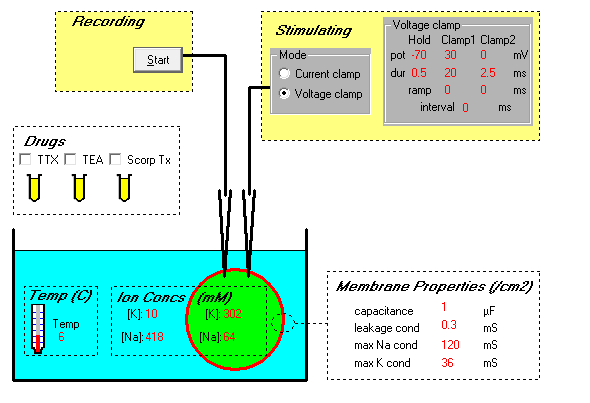
\includegraphics{images/Aufgabe3_1_Setup.png}
    \caption{Ausgangseinstellungen für Voltage Clamp Experiment}
    \label{fig:A3_1_Setup}
\end{figure}
\subsection{Bewegungswahrnehmung - Modul Networks}
In diesem Versuch wurden zwei neuronale Netzwerke modelliert, die Bewegung detektieren können.\\
Dazu wurde in Neurosim das Modul Networks geladen.
\subsubsection{Barlow-Levick}
Zunächst wurde ein neuronales Netz nach dem Barlow-Levick Modell erstellt.\\

\begin{figure}[H]
    \centering
    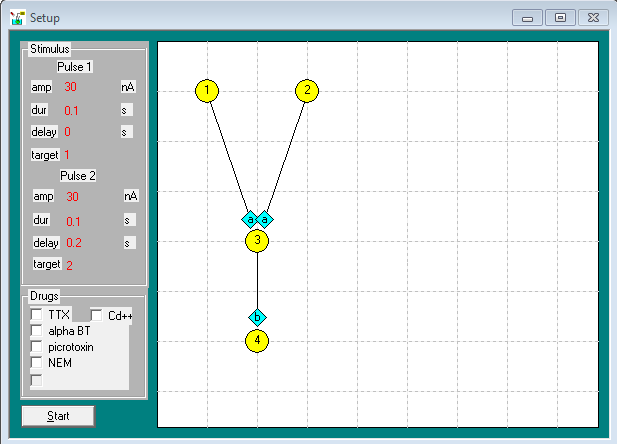
\includegraphics[scale=0.6]{images/Aufgabe4_1_Aufbau.png}
    \caption{Versuchsaufbau nach dem Barlow-Levick-Modell}
    \label{fig:A4_1_Aufbau}
\end{figure}
\newpage
\noindent Für die Wahrnehmung von Bewegung von links nach rechts wurde nach dem Barlow-Levick-Modell ein neuronales Netz bestehend aus 4 Neuronen(N1-N4) erzeugt. Abbildung \ref{fig:A4_1_Aufbau} zeigt den Aufbau grafisch. N1 liegt links von N2 und ist über eine erregende Synapse mit N3 verbunden. Die synaptische Verzögerung betrug 200ms. N2 ist ebenfalls über eine erregende Synapse mit N3 verbunden, allerdings ohne synaptische Verzögerung. N3 ist über eine hemmende Synapse mit N4 verbunden.\\ \\
Es wurden die Erregungen von N1 bis N4 gemessen, zunächst bei Simulation einer Bewegung von links nach rechts, anschließend von rechts nach links. Eine links-rechts Bewegung wird simuliert, indem zunächst ein Stimulus auf N1 gegeben wird, und mit 200ms Verzögerung auf N2. Für die rechts-links Bewegung wird zuerst N2 stimuliert, und N1 verzögert. Der Stimulus hatte eine Stromstärke von 30\(\mu\)A und eine Dauer von 100ms.\\
\subsubsection{Reichardt-Detektor}
Für den Versuchsaufbau für den Reichardt-Detektor wurde unsere Simulation um ein weiteres Neuron erweitert und die synaptischen Verbindungen, wie in Abbildung \ref{fig:A4_2_Aufbau} des Versuchsaufbaus zu sehen ist, verschaltet. Wie in der Abbildung zu sehen, sind N1 und N2 jeweils über Verbindungen gleichzeitig mit N3 und N4 verbunden. N3 und N4 hingegen haben jeweils eine Zielverbindung zu N5. 

\vspace{1.0\baselineskip}
\begin{figure}[H]
    \centering
    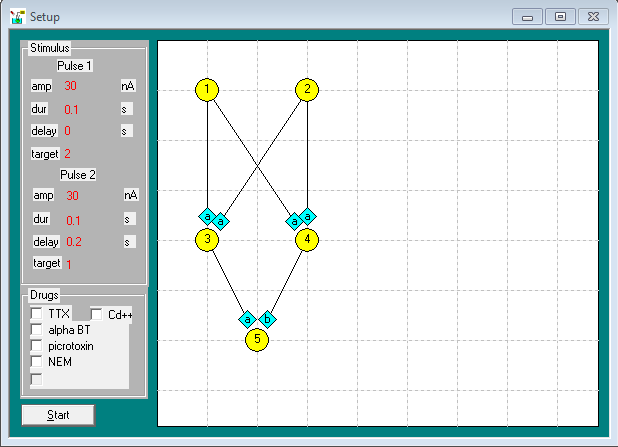
\includegraphics[scale=0.6]{images/Aufgabe4_2_Aufbau.png}
    \caption{Versuchsaufbau Reichardt-Hassenstein-Modell}
    \label{fig:A4_2_Aufbau}
\end{figure}

\noindent Um nun eine Bewegung von rechts nach links zu simulieren, wurde N1 so konfiguriert, dass es einen 100ms anhaltenden Impuls nach dem Starten der Simulation mit 200ms Verzögerung zu N2 abgibt. Für eine Bewegung von links nach rechts wurde analog zum Voraufbau die Verzögerung nun auf N2 konfiguriert.
Die Abbildung \ref{fig:A4_2_rechtsLinks} im Kapitel 3.4.2 zeigt die gemessene Spannung im Verlauf über ca. 600ms auf den Neuronen N1 - N5 bei der rechts-links Bewegung, \ref{fig:A4_2_linksRechts} eine links-rechts Messung. Der Parameter 'Initial Threshold' von N5 wurde auf -50mV gesetzt.Es wurden die Erregungen an allen 5 Neuronen für simulierte links-rechts und rechts-links Bewegungen gemessen.Weiterhin wurde die Impulsdauer gemessen, bei der nur noch ein Aktionspotential ausgelöst wurde. Im letzten Schritt wurde noch für unterschiedliche Reizschwellen an N3 die Anzahl der ausgelösten Aktionspotentiale gemessen.
\\
%
%\begin{figure}[H]
%    \centering
%    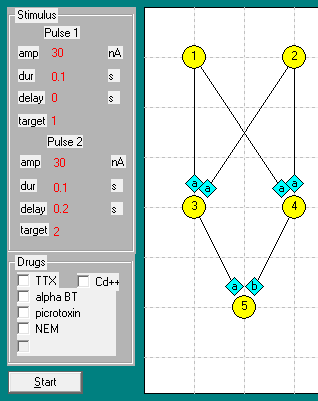
\includegraphics{images/Aufgabe4_2_Reichardt_Aufbau.png}
%    \caption{Verschaltung von Neuronen eines Reichardt-Detektors}
%    \label{fig:A4_2_Reich_Aufbau}
%\end{figure}

\newpage
\section{Ergebnisse}

\subsection{Modul Goldmann}
Bei steigender, extrazellulärer K\textsuperscript{+}-Konzentration wurde die Spannung für Membranpotential und Kaliumgleichgewichtspotential zunehmend positiver.
\begin{figure}[H]
    \centering
    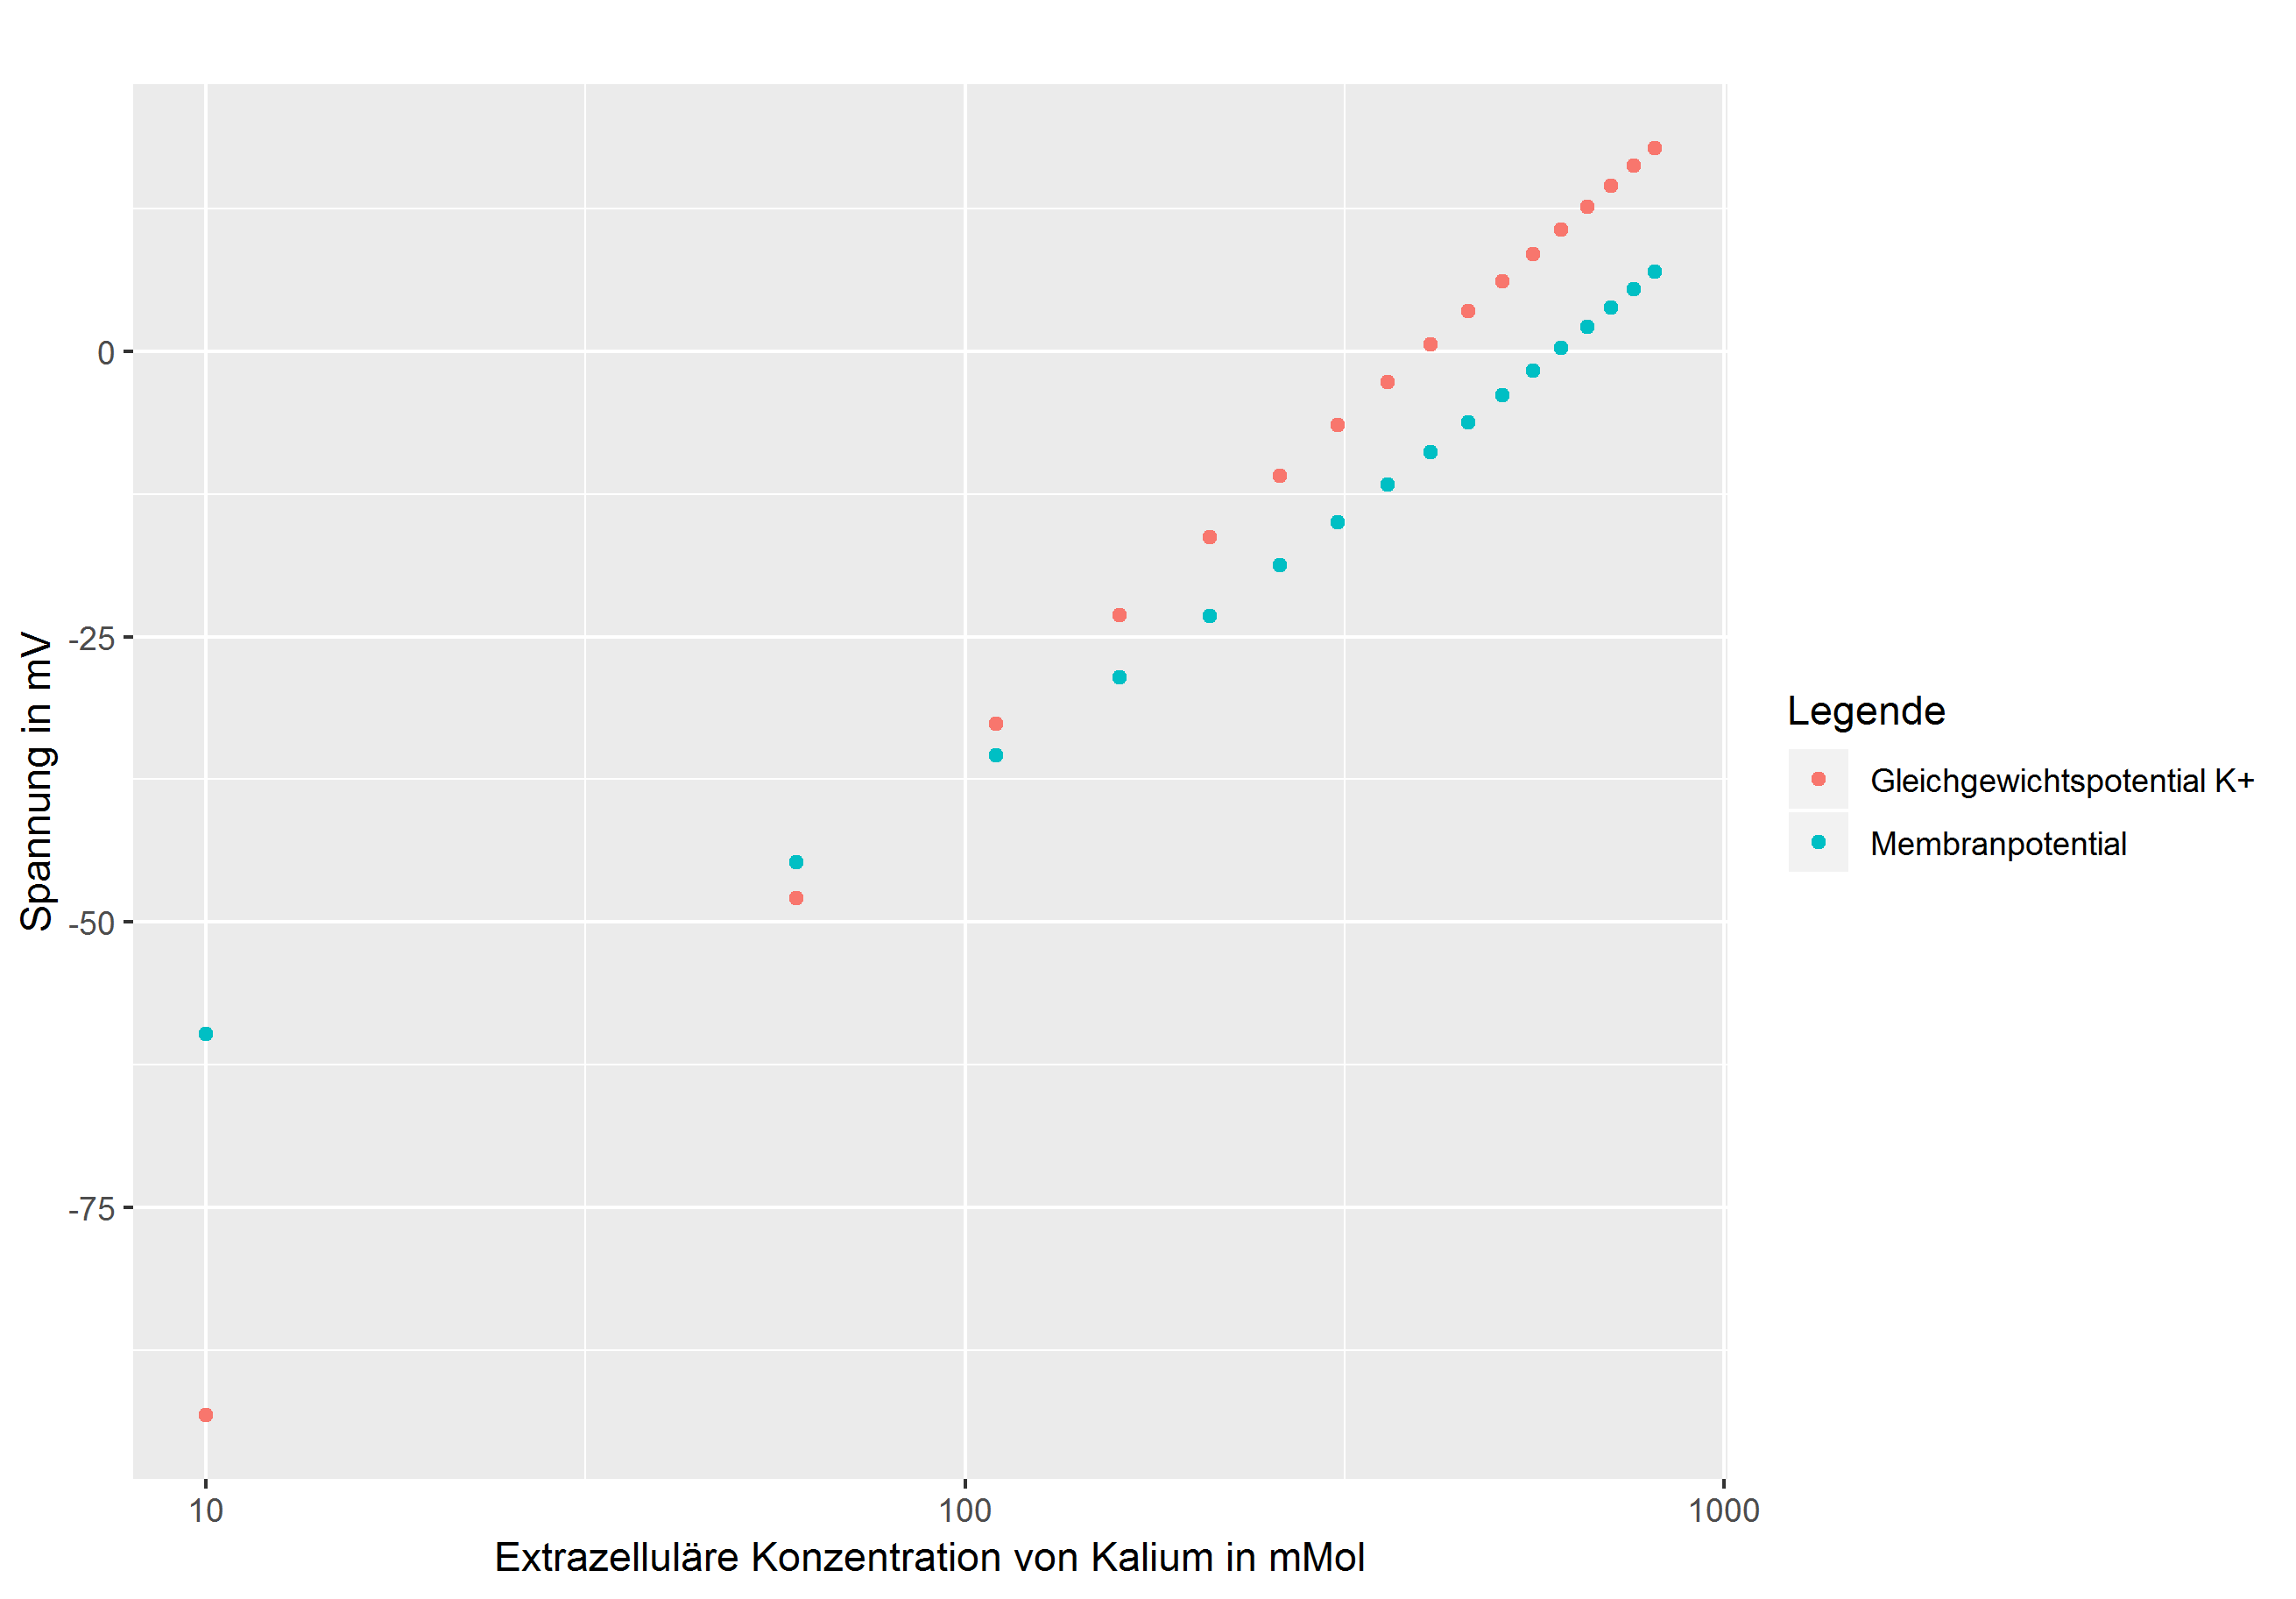
\includegraphics[width=\textwidth]{images/Aufgabe1_3.png}
    \caption{Spannungsänderung bei zunehmender Kaliumkonzentration (extrazellulär)}
    \label{fig:A1_2}
\end{figure}

\noindent Für beispielhafte Werte in Tabelle \ref{tab:A1_4} ergab sich nach der Goldmann-Gleichung ein Membranpotenzial von -51.35 mV. Die sich laut der Nernst'schen Gleichung ergebenden Gleichgewichtspotentiale E\textsubscript{ion} sind mit in der Tabelle dargestellt.
\begin{table}[H]
    \centering
    \caption{Beispielwerte zur Berechnung eines Membranpotentials}
    \begin{tabular}{|c|c|c|c|c|}
        \hline
        \textbf{Ion} & \textbf{Relative Permeabilität} & \textbf{Konz. innen} & \textbf{Konz. außen} & \textbf{E\textsubscript{ion}}\\
        \hline
        K\textsuperscript{+} & 1.0 & 124 & 4 & -86.5\\
        \hline
        Na\textsuperscript{+} & 0.04 & 50 & 470 & +56.4\\
        \hline
        Cl\textsuperscript{-} & 0.3 & 55 & 580 & +59.3\\
        \hline
    \end{tabular}
    \label{tab:A1_4}
\end{table}

\newpage
\subsection{Modul Hodgkin-Huxley (Current Clamp)}

Das erste Aktionspotential wurde bei 40.74\(\mu\)A beobachtet.\\
Bei der schrittweisen Erhöhung der Stromstärke um 10\(\mu\)A stieg die Maximalspannung, wie in  Tabelle \ref{tab:A2_3} erkennbar, bis 70.74\(\mu\)A an, und blieb dann weitgehend konstant. Die Dauer bis zum Spannungsmaximum verkürzte sich mit Erhöhung der Stromstärke, flachte aber auch zunehmend ab.

\vspace{2.5\baselineskip}

\begin{table}[H]
    \centering
    \caption{Spannungsänderung in Bezug zur Stromstärke}
    \begin{tabular}{c||c|c}
        Stromstärke (\(\mu\)A) & Maximalspannung (mV) & Dauer bis Maximalspannung (ms)\\
        \hline
        40,74 & -13,33 & 2,86 \\
        50,74 & 25,00 & 1,33\\
        60,74 & 28,33 & 1,12\\
        70,74 & 31,67 & 1,05\\
        80,74 & 30,00 & 0,96\\
        90,74 & 31,67 & 0,94\\
    \end{tabular}
    \label{tab:A2_3}
\end{table}

\begin{table}[H]
    \centering
    \caption{Änderung von Frequenz und Amplitude in Bezug zur Stromstärke}
    \begin{tabular}{c||c|c}
        Stromstärke (\(\mu\)A) & Frequenz (Hz) & 1. Amplitude (mV) \\
        \hline
        2 & 10 & 30\\
        7 & 60 & 35\\
        12 & 70 & 35\\
        22 & 90 & 35\\
        32 & 100 & 35\\
        42 & 110 & 36,67\\
        67 & 120 & 36,67\\
        92 & 140 & 38,33\\
        117 & 140 & 40\\
        130 & 40 & 38,33
    \end{tabular}
    \label{tab:A2_4}
\end{table}

\vspace{2.5\baselineskip}

\noindent Wie in Abbildung \ref{fig:A2_4} zu sehen, nahm die erste Amplitude zwar mit steigender Stromstärke zu, allerdings verloren die Folgeamplituden zunehmend das charakteristische Aussehen eines Aktionspotentials.\\

\begin{figure}[H]
    \centering
    \begin{tabular}{|c|}
        \hline
         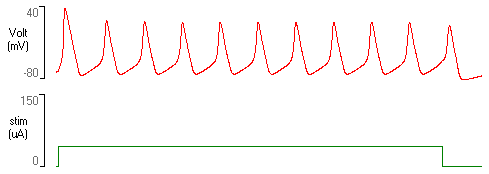
\includegraphics{images/Aufgabe2_4_amp42_Amps.png} \\
         \hline
         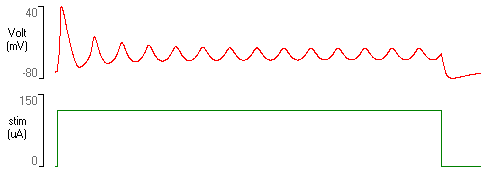
\includegraphics{images/Aufgabe2_4_amp117_Amps.png}\\
         \hline
         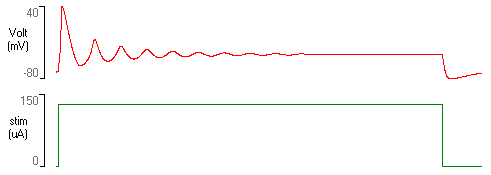
\includegraphics{images/Aufgabe2_4_amp130_Amps.png}\\
         \hline
    \end{tabular}
    \caption{Änderung in den Folgeamplituden bei steigender Stromstärke}
    \label{fig:A2_4}
\end{figure}

\subsection{Modul Hodgkin-Huxley (Voltage Clamp)}
% TODO: Beschreibung zu Aufgabe 3.2
Bei einer Haltespannung von -70mV und einer Klemmspannung von +30mV ließ sich, wie in Abbildung \ref{fig:A3_2} gezeigt, eine logarithmisch verlaufende Stromkurve beobachten.\\ \\
Beim Blocken von Kaliumkanälen mittels TEA ließ sich der isolierte Natriumstrom beobachten, zu sehen in Abbildung \ref{fig:A3_3a}. Die Stromstärke wurde anfangs negativer, und nähert sich langsam wieder dem Ausgangsniveau.\\ \\
Beim Blocken von Natriumkanälen mittels TTX ließ sich der isolierte Kaliumstrom beobachten, zu sehen in Abbildung \ref{fig:A3_3b}. Die Kurve zeigte einen raschen Ausstrom von Kalium, der langsam ein Maximum annahm.\\ \\
In Abbildung \ref{fig:A3_4} ist gezeigt, wie die Ströme bei zunehmender Klemmspannung verliefen. Der Kaliumstrom begann bei +93.75\(\mu\)A und stieg bis +4265.63\(\mu\)A. Der Natriumstrom sank von -328.13\(\mu\)A bis auf -2390.63\(\mu\)A bei -10mV und stieg von dort an wieder, bis auf +328.13\(\mu\)A.\\ \\
Abbildung \ref{fig:A3_4a} und \ref{fig:A3_4b} zeigen die Verläufe der isolierten Kalium- und Natriumströme.
\begin{figure}[H]
    \centering
    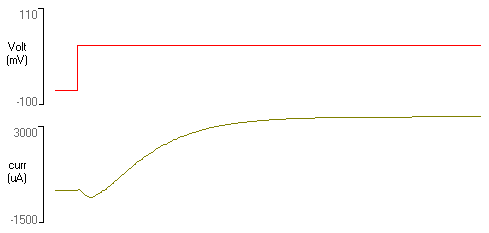
\includegraphics{images/Aufgabe3_2.png}
    \caption{Gesamtstrom bei Haltespannung -70mV und Klemmspannung +30mV}
    \label{fig:A3_2}
\end{figure}
\begin{figure}[H]
  \centering
  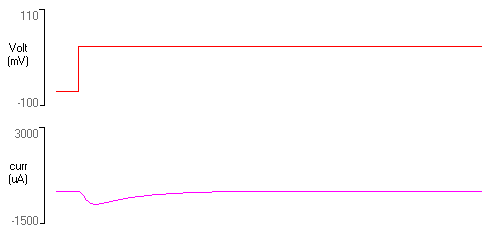
\includegraphics{images/Aufgabe3_3-TEA_Na_Detail.png}
  \caption{Isolierter Natriumstrom durch Blocken der Kaliumkanäle mit TEA}
  \label{fig:A3_3a}
\end{figure}
\begin{figure}[H]
  \centering
  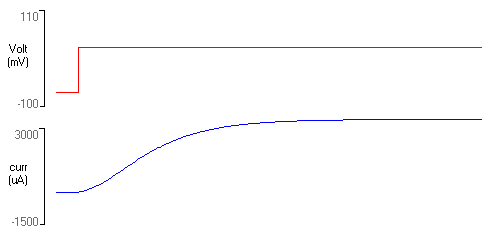
\includegraphics{images/Aufgabe3_3-TTX_K_Detail.png}
  \caption{Isolierter Kaliumstrom durch Blocken der Natriumkanäle mit TTX}
  \label{fig:A3_3b}
\end{figure}
\begin{figure}[H]
    \centering
    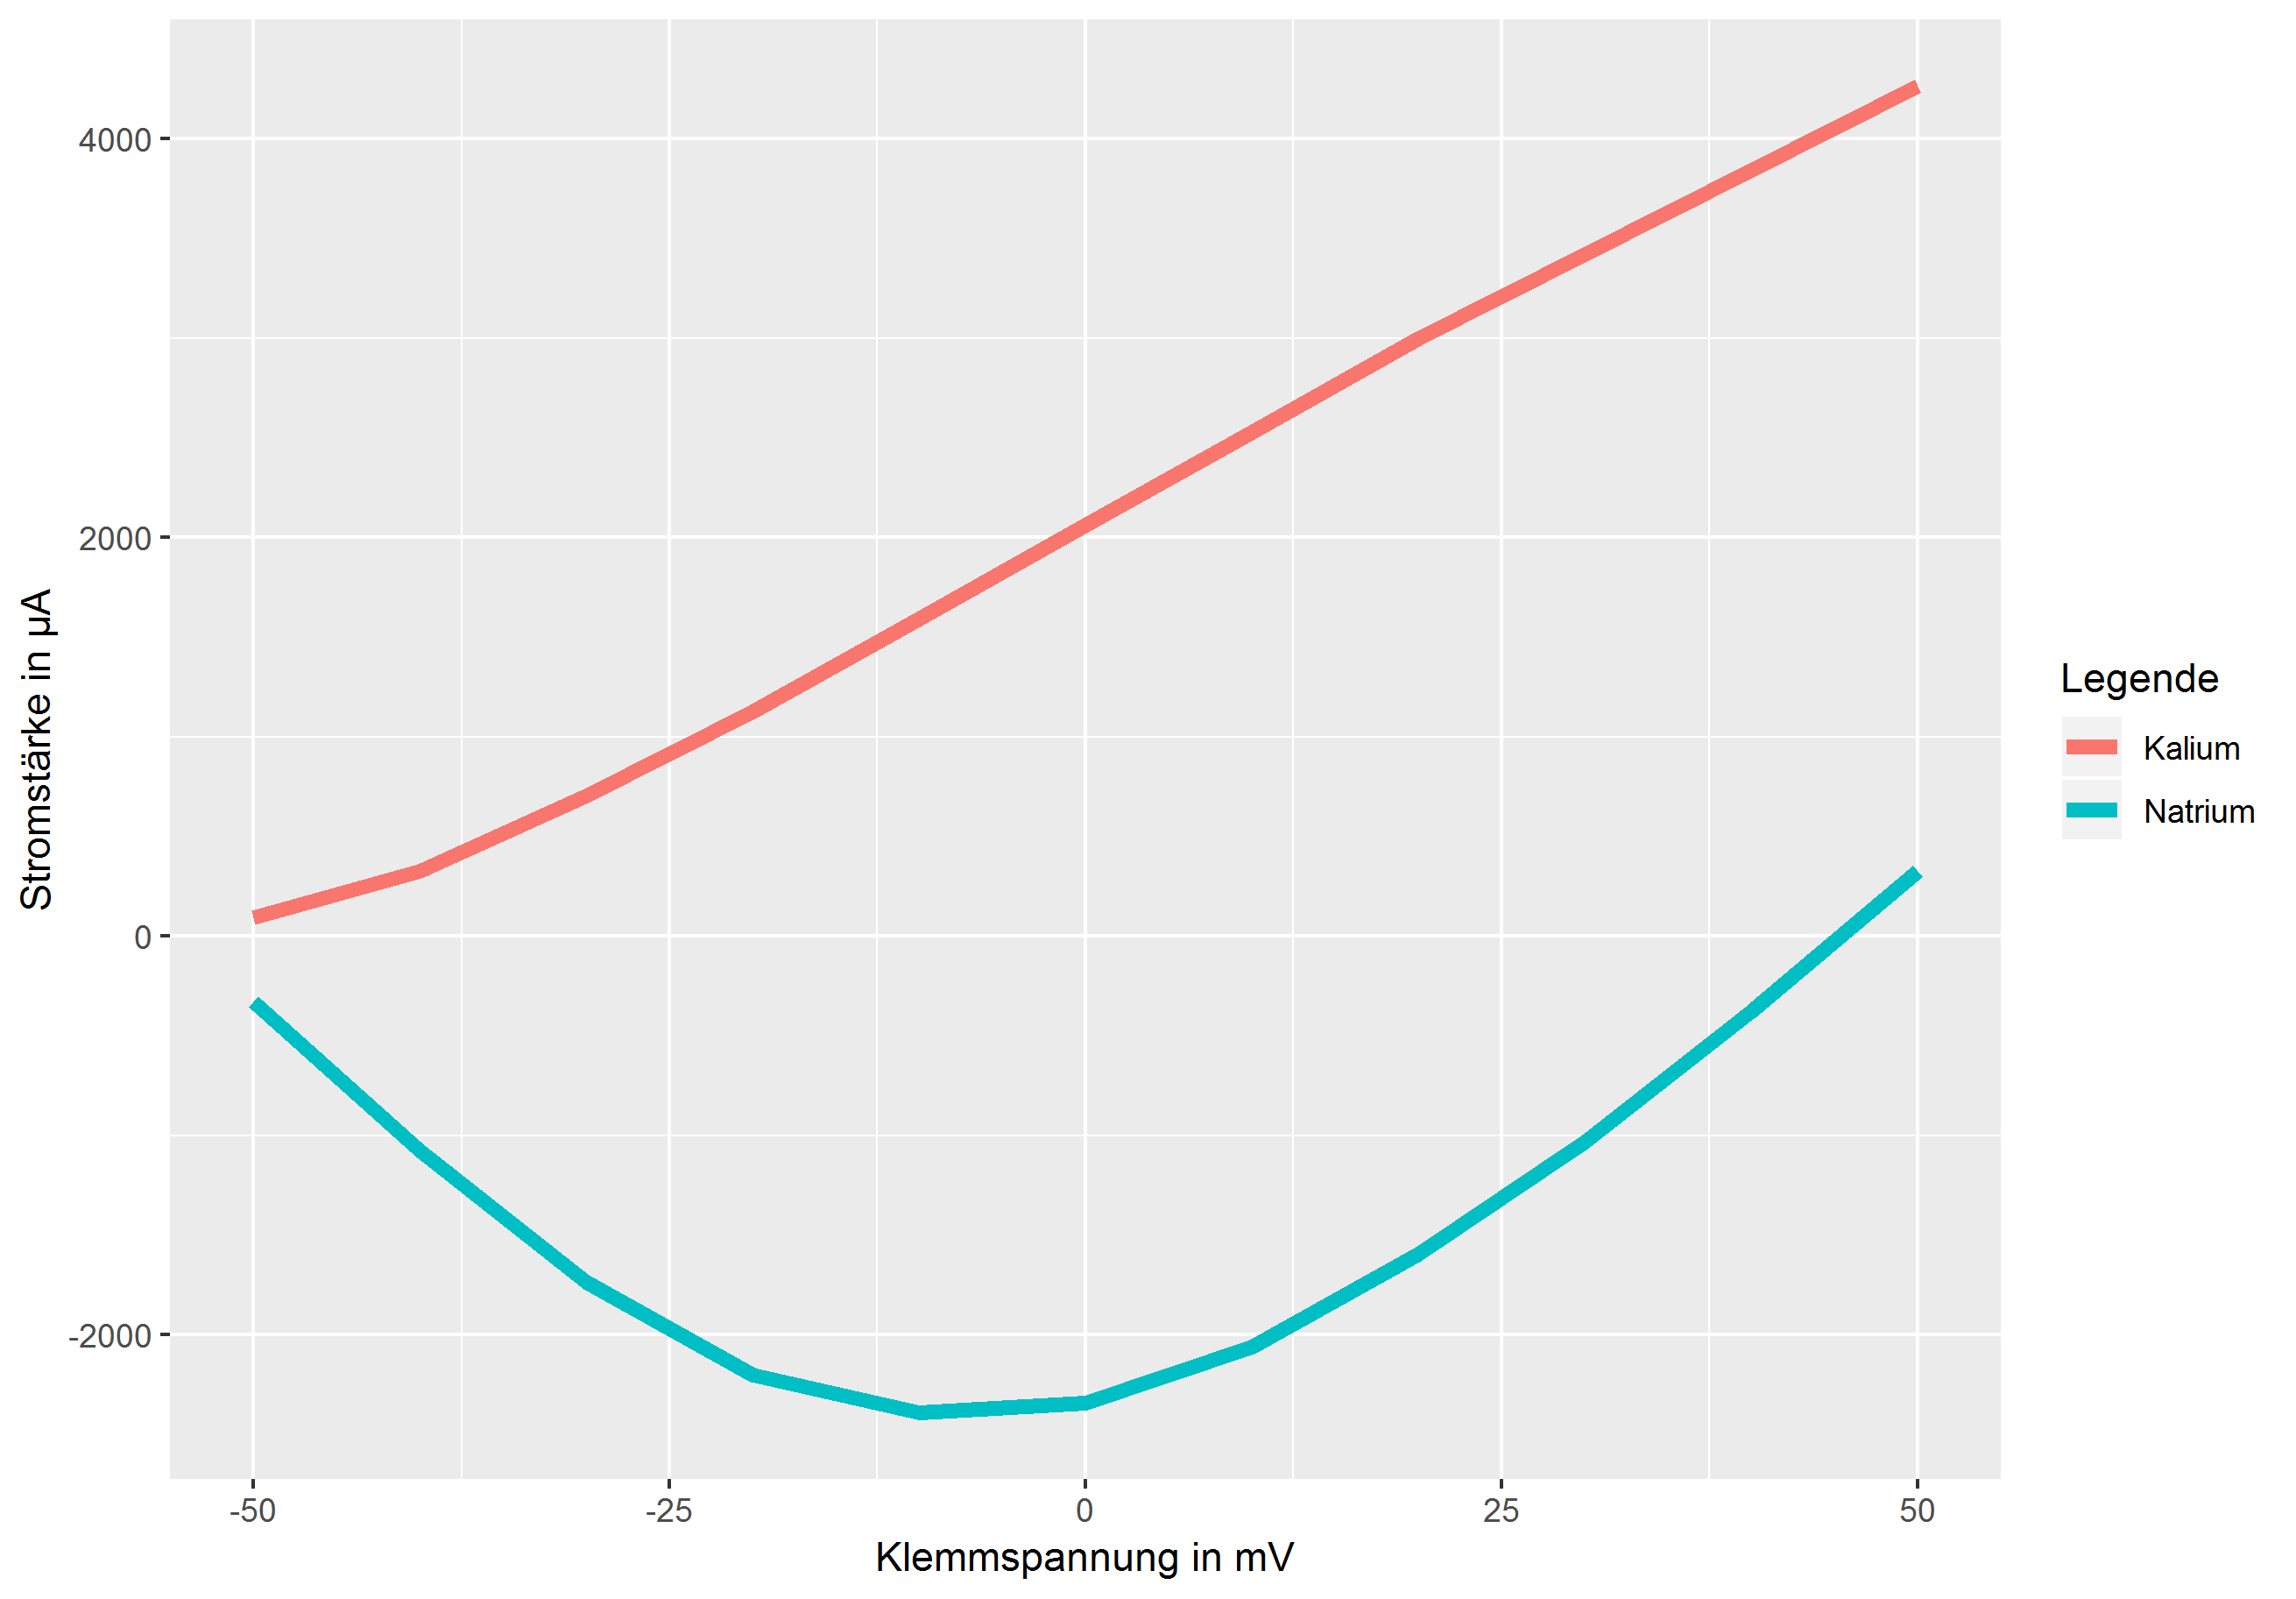
\includegraphics[width=\textwidth]{images/Aufgabe3_4.png}
    \caption{Stromstärken I\textsubscript{Na} und I\textsubscript{K} in Bezug zur Klemmspannung}
    \label{fig:A3_4}
\end{figure}
\begin{figure}[H]
    \centering
    \begin{tabular}{|c|}
        \hline
         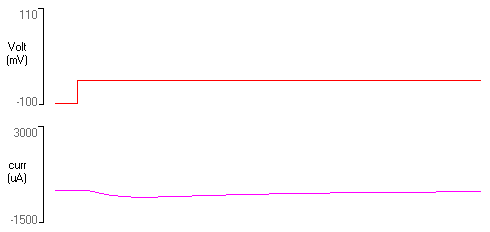
\includegraphics{images/Aufgabe3_4-ClampMinus50-TEA_Graph.png} \\
         \hline
         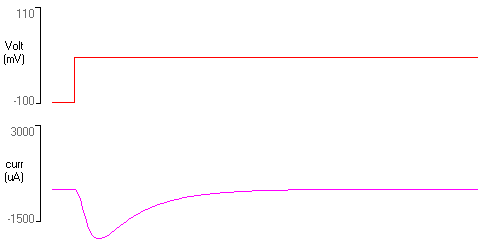
\includegraphics{images/Aufgabe3_4-Clamp0-TEA_Graph.png}\\
         \hline
         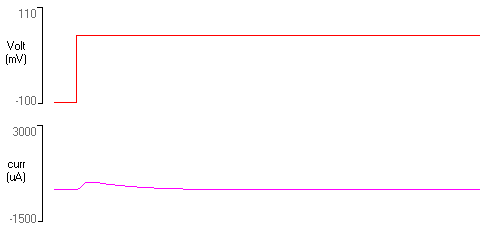
\includegraphics{images/Aufgabe3_4-Clamp50-TEA_Graph.png}\\
         \hline
    \end{tabular}
    \caption{Isolierte Natriumströme bei -50mv, 0mv, bzw. +50mV Klemmspannung, und +100mV Haltespannung.}
    \label{fig:A3_4a}
\end{figure}
\begin{figure}[H]
    \centering
    \begin{tabular}{|c|}
        \hline
         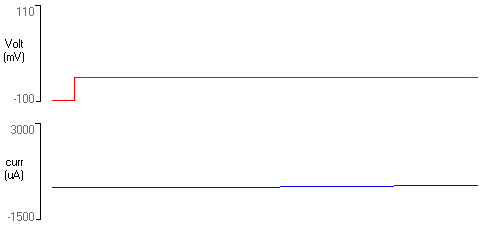
\includegraphics{images/Aufgabe3_4-ClampMinus50-TTX_Graph.png} \\
         \hline
         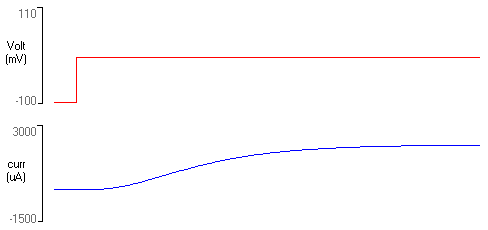
\includegraphics{images/Aufgabe3_4-Clamp0-TTX_Graph.png}\\
         \hline
         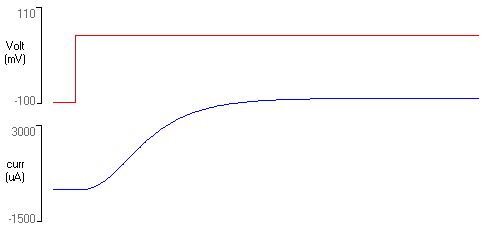
\includegraphics{images/Aufgabe3_4-Clamp50-TTX_Graph.png}\\
         \hline
    \end{tabular}
    \caption{Isolierte Kaliumströme bei -50mv, 0mv, bzw. +50mV Klemmspannung und +100mV Haltespannung.}
    \label{fig:A3_4b}
\end{figure}

\newpage
\subsection{Bewegungswahrnehmung}
\subsubsection{Barlow-Levick-Modell}

%Kurze Beschreibung für Aufgabe 4.1
\noindent Die Spannungsänderungen an Neuronen für eine links-rechts Bewegung sieht man in Abbildung \ref{fig:A4_1a}.
Bei Simulation eines Reizes, der zuerst N1 und um 200ms verzögert N2 stimulierte (links-rechts Bewegung), wurden an N3 Aktionspotentiale ausgelöst. An N4 war eine Hyperpolarisierung zu beobachten. \\ \\
Die Spannungsänderungen an Neuronen für eine rechts-links Bewegung sieht man in Abbildung \ref{fig:A4_1b}. Bei Simulation eines Reizes, der zuerst N2 und um 200ms verzögert N1 stimulierte, waren an N3 unterschwellige Spannungsänderungen erkennbar, allerdings keine Aktionspotentiale. An N4 konnten  keine Spannungsänderungen beobachtet werden. 
\\
\begin{figure}[H]
    \centering
    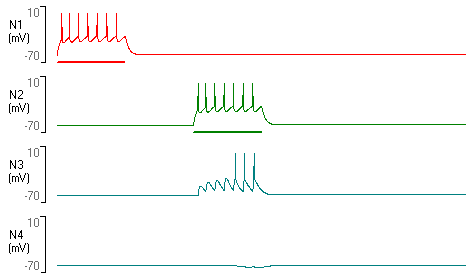
\includegraphics[scale=0.7]{images/Aufgabe4_1_linksRechts.png}
    \caption{Beobachtete Spannungen an Neuronen N1-N4 \\ bei Bewegung von links nach rechts}
    \label{fig:A4_1a}
\end{figure}

\vspace{2.0\baselineskip}

\begin{figure}[H]
    \centering
    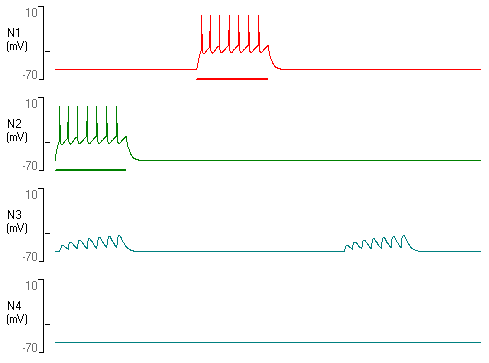
\includegraphics[scale=0.7]{images/Aufgabe4_1_rechtsLinks.png}
    \caption{Beobachtete Spannungen an Neuronen N1-N4 \\ bei Bewegung von rechts nach links}
    \label{fig:A4_1b}
\end{figure}

\newpage
\subsubsection{Reichardt-Hassenstein-Modell}
Die Abbildung \ref{fig:A4_2_linksRechts} zeigt die gemessene Spannung bei einer links-rechts Bewegung, die Abbildung \ref{fig:A4_2_rechtsLinks} die Messungen bei der rechts-links Bewegung. Auf der x-Achse der jeweiligen Abbildungen sind die einzelnen Neuronen verzeichnet und ihrer jeweilige Wert in mV. Die y-Achse verzeichnet die Messdauer in Sekunden. Der Ausschnitt unserer abgebildeten Messungen beschränkte sich auf ca. 600ms. Bei dem direkten Vergleich beider Messungen ist zu sehen, dass es nur bei der in Abbildung \ref{fig:A4_2_linksRechts} zu sehenden links-rechts Bewegung tatsächlich zu einer Aktivierung des N5 Neurons kommt. 
\vspace{2.0\baselineskip}
\begin{figure}[H]
    \centering
    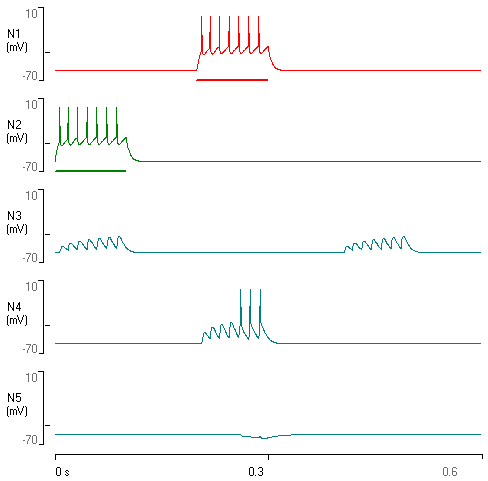
\includegraphics[scale=0.7]{images/Aufgabe4_2_rechtsLinks.png}
    \caption{Simulierte Bewegung von rechts nach links}
    \label{fig:A4_2_rechtsLinks}
\end{figure}

\begin{figure}[H]
    \centering
    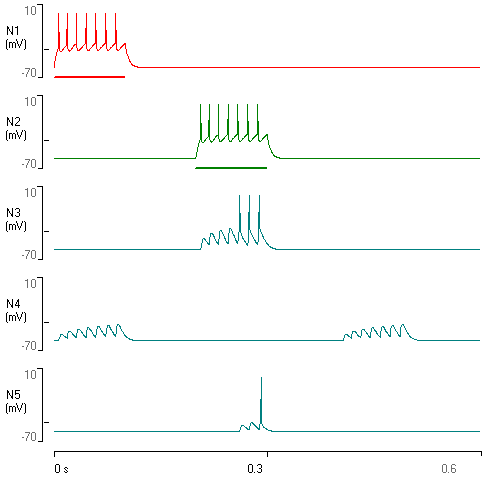
\includegraphics[scale=0.7]{images/Aufgabe4_2_linksRechts.png}
    \caption{Simulierte Bewegung von links nach rechts}
    \label{fig:A4_2_linksRechts}
\end{figure}

%Zu 4.4c
\newpage
\noindent Bei Änderung der Reizschwelle an N3 konnten die in Tabelle \ref{tab:A4_4c} dargestellten Aktionspotentiale gemessen werden. Je negativer die Reizschwelle, desto mehr Aktionspotentiale wurden ausgelöst. Zudem wurde beobachtet, dass ab einer Reizschwelle von -46mV bereits einseitige Erregung von N1 oder N2 ausreichte um ein Aktionspotential an N3 auszulösen. \vspace{1}

\begin{table}[H]
    \centering
    \caption{Aktionspotentiale an N3 bei Änderung der Reizschwelle}
    \begin{tabular}{c|c}
         Reizschwelle & Anzahl Aktionspotentiale  \\
         \hline
         -50 & 7\\
         -45 & 6\\
         -42 & 4\\
         -40 & 3\\
         -38 & 1\\
         -37 & 0\\
         -30 & 0
    \end{tabular}
    \label{tab:A4_4c}
\end{table}

\newpage
\section{Diskussion}
\vspace{1.0\baselineskip}
\subsection{Modul Goldmann}
Bei zunehmender extrazellulärer Kaliumkonzentration konnte beobachtet werden, dass \\  K\textsuperscript{+}-Gleichgewichtspotential und Membranpotential zunehmend positiv wurden.
Dies bestätigt unsere durch die Goldmann-Gleichung gegebenen Erwartungen. Wenn die extrazelluläre Kaliumkonzentration \([K^+]_o\) im Nenner steigt, wird das Ergebnis der Gleichung positiver.

\subsection{Modul Hodgkin-Huxley (Current Clamp)}
Bei steigender Stromstärke konnte beobachtet werden, dass die Maximalspannung ab einem gewissen Punkt einen Maximalwert erreicht. Wir schließen daraus, dass ab diesem Punkt alle verfügbaren Natriumkanäle sofort geöffnet werden.\\ \\
Zu beobachten war auch, dass ab einer gewissen Stromstärke keine vollständigen Folgepotentiale mehr ausgebildet werden. Da durch die starke Depolarisierung die spannungsaktivierten Kaliumkanäle geöffnet bleiben, nimmt das Membranpotential einen negativeren Wert an, d.h. die positiven Spitzen der Aktionspotentiale sind geringer.

\subsection{Modul Hodgkin-Huxley (Voltage Clamp)}
Die beobachtete Steigung des Kaliumstroms kann durch den bereits existiernden Konzentrationsgradienten erklärt werden. Je positiver die Spannung im Zellinneren wird, desto mehr werden Kaliumionen auch durch den Spannungsgradient nach außen befördert.\\
Der Verlauf des Natriumstroms ist auf gleiche Weise erklärbar. Zunächst führt der die geringe Natriumkonzentration in der Zelle dazu, dass Natrium einströmt. Mit zunehmender positiver Spannung wird durch den Spannungsgradient der Natriumeinstrom vermindert, und wird über dem Gleichgewichtspotential von ca. +47mV zu einem Natriumausstrom.
\subsection{Bewegungswahrnehmung}
\vspace{1.0\baselineskip}
% Zu Aufgabe 4.1:
\subsubsection{Barlow-Levick-Modell} 
Wie erwartet werden an N3 nur Aktionspotentiale erzeugt, wenn die APs aus N1 und N2 zeitgleich eintreffen. Durch die Summation der beiden APs kann der Schwellwert an N3 überschritten, und APs Richtung N4 geleitet werden.
\subsubsection{Reichardt-Hassenstein-Modell}
Über dieses Modell konnte gezeigt werden, dass es mithilfe des Reichardt-Detektor möglich ist, durch eine simulierte Bewegung in eine bestimmte Richtung das Feuern eines Neurons zu erreichen. Hierbei wird der Detektor nur aktiviert, wenn der Reiz zuerst an N1 und dann mit Verzögerung bei N2 eintrifft (s. Abb. \ref{fig:A4_2_linksRechts}, Kapitel 3.4.2). Bei einer umgekehrten Reizung (s. Abb. \ref{fig:A4_2_rechtsLinks}, Kapitel 3.4.2) wird der Detektor hingegen gehemmt. Der Detektor wird also abhängig von der Verzögerung der Reize an N1 und N2 gefeuert, was bedeutet, dass für jede Bewegungen mit unterschiedlicher Geschwindigkeit ein Detektor abgebildet werden muss.

\newpage
\printbibliography

\end{document}